\documentclass{article}

\usepackage[letterpaper,top=1cm,bottom=1cm,left=2cm,right=2cm,marginparwidth=1.75cm]{geometry}

\usepackage{tikz}
\usepackage{amsmath}
\usepackage{siunitx}
\usepackage{multicol}

\newcommand*\circled[1]{\tikz[baseline=(char.base)]{\node[shape=circle,draw,inner sep=2pt] (char) {#1};}}

\newcommand*\mss{\unit{m/s^2}}

\newcommand*\VecUnit[2]{\unit{#1}[#2]}

\newcommand*\Kg{\unit{kg}}
\newcommand*\N{\unit{N}}

\begin{document}

            \center{\section*{Going up}}
\begin{multicols}{2}

    \center{\underline{\circled{1} {Givens}}}

    \begin{equation*}
        \begin{aligned}
            &m_{cab} = 1360 \Kg\\
            &m_{capacity} = 1200 \Kg\\
            &m_T = m_{cab} + m_{capacity} = 1360\Kg + 1200\Kg = 2560 \Kg\\
            &\vec{a}_{su} = 0.2\mss[U]\\
            &\vec{a}_{sd} = 0.6\mss[D]\\
            &\vec{g} = 9.81\mss[D]\\
        \end{aligned}
    \end{equation*}

    \center{\underline{\circled{2} {Rearrange}}}
    \begin{equation*}
        \begin{aligned}
            \Sigma \vec{F} &= \vec{F}_{net}\\
            \vec{F}_{net} &= \vec{F}_g + \vec{F}_t\\
            \vec{F}_g + \vec{F}_t &= m\vec{a}\\
            \vec{F}_t &= m\vec{a} - \vec{F}_{g}\\
            \vec{F}_t &= m\vec{a} - m\vec{g}
        \end{aligned}
    \end{equation*}

    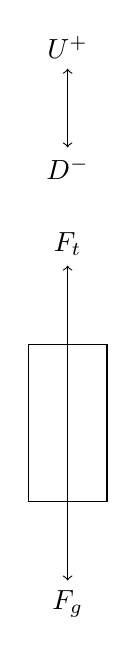
\begin{tikzpicture}
        \draw[<->] (0,3.5) coordinate (down) -- (0, 4.5) coordinate (up);
    
        \node at (up)[anchor=south] {$U^+$};
        \node at (down)[anchor=north] {$D^-$};

        \draw (-0.5, -1) rectangle (0.5, 1);

        \draw[->] (0, 0) -- ++ (0, 2) node [anchor=south]{$F_t$};
        \draw[->] (0, 0) -- ++ (0, -2) node [anchor=north]{$F_g$};
    \end{tikzpicture}

\end{multicols}

    \begin{multicols}{2}
        \center{\underline{\circled{3} {Solve for speeding up}}}
        \begin{equation*}
            \begin{aligned}
                \vec{F}_t &= m_T\vec{a}_{su} - m\vec{g}\\
                \vec{F}_t &= (2560 \Kg)(0.2\mss) - (2560\Kg)(-9.81\mss)\\
                \vec{F}_t &= (512 \N) - (-25113.6\N)\\
                \vec{F}_t &= 25625.6\N\\
            \end{aligned}
        \end{equation*}

        \fbox {$\vec{F}_{t} = 25625.6 \VecUnit{N}{U} $}

        \center{\underline{\circled{4} {Solve for slowing down}}}
        \begin{equation*}
            \begin{aligned}
                \vec{F}_t &= m_T\vec{a}_{sd} - m\vec{g}\\
                \vec{F}_t &= (2560 \Kg)(-0.6\mss) - (2560\Kg)(-9.81\mss)\\
                \vec{F}_t &= (-1536\N) - (-25113.6\N)\\
                \vec{F}_t &= 26649.6\N\\
            \end{aligned}
        \end{equation*}

        \fbox {$\vec{F}_{t} = 26649.6 \VecUnit{N}{U} $}

    \end{multicols}
\end{document}
